%\motto{Use the template \emph{chapter.tex} to style the various elements of your chapter content.}
\chapter{Anwendungsgebiete im Finanzbereich}
\label{trends} % Always give a unique label
% use \chaptermark{}
% to alter or adjust the chapter heading in the running head

\chapterauthor{Lola Bankai, Felix Goos}

\abstract{Dieses Kapitel untersucht das Potenzial von Quantencomputing für den Einsatz im Finanzwesen. Im Zentrum stehen drei besonders rechenintensive Anwendungsfelder: Portfoliooptimierung, Monte-Carlo-Simulationen und Risikomessung. Anhand aktueller Forschungsergebnisse und Pilotprojekte wird analysiert, wie Quantenalgorithmen klassische Verfahren ergänzen oder perspektivisch ablösen könnten. Dabei werden sowohl Quantum Annealing als auch gate-basierte Algorithmen wie QAOA, VQE und QAE betrachtet. Darüber hinaus beleuchtet das Kapitel die Rolle führender Technologieunternehmen, Finanzinstitute und internationaler Forschungsinitiativen. Abschließend erfolgt eine kritische Bewertung der technologischen Entwicklungen mit Blick auf konkrete Einsatzmöglichkeiten, bestehende Herausforderungen und strategische Implikationen für die Finanzbranche.}

\section{Einleitung}
Das Finanzwesen zählt zu den datenintensivsten und rechentechnisch anspruchsvollsten Bereichen der modernen Wirtschaft. Täglich werden riesige Datenmengen analysiert, komplexe Modelle berechnet und Entscheidungen unter Unsicherheit getroffen. Klassische Computersysteme stoßen hierbei zunehmend an ihre Leistungsgrenzen, insbesondere wenn es um die Lösung kombinatorischer Optimierungsprobleme, stochastischer Simulationen oder die Verarbeitung hochdimensionaler Datenstrukturen geht. In diesem Kontext rücken Quantencomputer als potenziell transformative Technologie in den Fokus. Sie beruhen auf den Prinzipien der Quantenmechanik wie Superposition, Verschränkung und Interferenz und ermöglichen damit neue Arten der Informationsverarbeitung, die bei bestimmten Problemklassen eine exponentielle Beschleunigung gegenüber klassischen Verfahren versprechen.

Erste Forschungsarbeiten und Pilotprojekte belegen, dass Quantenalgorithmen insbesondere in der Portfoliooptimierung, in der Bewertung komplexer Finanzinstrumente sowie im Risikomanagement erhebliche Vorteile bringen könnten. Dabei geht es nicht nur um Rechengeschwindigkeit, sondern auch um die Möglichkeit, realistischere Modelle zu verwenden, die bislang aufgrund ihrer Komplexität nicht praktikabel waren. Gleichzeitig stellt die wachsende Leistungsfähigkeit von Quantencomputern auch eine Bedrohung für klassische kryptografische Verfahren dar, was die Notwendigkeit neuer Sicherheitsstrategien aufwirft.

Im weiteren Verlauf dieses Kapitels werden zunächst die zentralen Herausforderungen und Chancen des Quantencomputings im Finanzwesen dargestellt. Anschließend werden die drei wichtigsten Anwendungsfelder beleuchtet: Portfoliooptimierung, Optionsbewertung und Risikomessung. Darauf folgt eine Übersicht über die zugrunde liegenden Technologien und Algorithmen. Zudem werden führende Akteure, bedeutende Unternehmensinitiativen sowie ausgewählte Forschungsprojekte vorgestellt. Den Abschluss bildet eine Bewertung der Entwicklungen und ein Teilfazit mit Blick auf zukünftige Potenziale.

\section{Relevanz und Problemstellung}
Zu den datenintensivsten und rechenaufwendigsten Bereichen der modernen Wirtschaft zählt das Finanzwesen. Jeden Tag müssen enorme Datenmengen ausgewertet, komplizierte Modelle beurteilt und Entscheidungen mit Risiko getroffen werden   häufig unter Bedingungen von Unsicherheit und in dynamischen Märkten. Bei der Bewältigung solcher Aufgaben geraten herkömmliche Computer zunehmend an ihre Grenzen. Der Rechenaufwand in Bereichen wie Optimierung, Simulation oder probabilistischer Risikobewertung wächst insbesondere mit der Komplexität von Finanzprodukten und -märkten exponentiell an \cite{springer2025,plos2024}.

Quantencomputer stellen ein neuartiges Paradigma dar: Sie verarbeiten Informationen auf der Grundlage quantenmechanischer Zustände, was die parallele Bearbeitung bestimmter mathematischer Probleme mit einem erheblichen Geschwindigkeitsvorteil ermöglicht. Neue Lösungsräume eröffnen sich insbesondere bei kombinatorischen Optimierungsproblemen, wie sie beispielsweise in der Portfoliozusammensetzung oder im Optionspricing vorkommen, sowie bei stochastischen Simulationen. Erste Untersuchungen haben ergeben, dass Quantenalgorithmen diese Aufgaben mit einer deutlich höheren Effizienz bewältigen können als klassische Verfahren \cite{quantumjournal2020,orus2019}.

Zugleich bringt die Verwendung von Quantencomputern im Finanzsektor neue Herausforderungen mit sich. Vor allem die Gefahr, dass klassische kryptographische Verfahren brechen könnten, steht neben der noch nicht voll ausgereiften Hardware im Raum. Es geht dabei nicht nur um den Schutz sensibler Finanzdaten, sondern auch um die Stabilität ganzer Systeme. Das sogenannte „Harvest Now, Decrypt Later“-Szenario ist besonders kritisch. Dabei werden heute verschlüsselte Daten abgefangen, um sie später mit leistungsfähigen Quantencomputern zu entschlüsseln \cite{finance21net}.

Damit befindet sich der Finanzsektor an einem Wendepunkt: Auf der einen Seite bieten Quantencomputer enorme Möglichkeiten zur Effizienzsteigerung und zur Verbesserung bestehender Verfahren   wie bei Risikomodellen, Investmentstrategien oder der Integration mit künstlicher Intelligenz \cite{finance21net}. Auf der anderen Seite ist es notwendig, dass bestehende Infrastrukturen rechtzeitig gegen neue Bedrohungen geschützt werden. Die Chance-Risiko-Dualität macht Quantencomputing für den Finanzsektor äußerst relevant und zeigt die Notwendigkeit praxisnaher Forschung und strategischer Vorausschau auf \cite{springer2025,orus2019}.

!!hier fehlen noch die dinger in zotero

\section{Top 3 Anwendungsfelder (Praxis \& Theorie)}

Die konkrete Anwendbarkeit von Quantencomputern im Finanzsektor lässt sich exemplarisch an drei besonders rechenintensiven und praxisrelevanten Bereichen aufzeigen. Diese Felder zeichnen sich durch hohe algorithmische Komplexität und umfangreiche Datenanforderungen aus und gelten daher als vielversprechende Einsatzgebiete für quantenbasierte Verfahren. Im Folgenden wird untersucht, in welchem Ausmaß Quantenalgorithmen klassische Methoden ergänzen oder perspektivisch ablösen könnten.

Die drei zentralen Anwendungsfelder sind:

\begin{itemize}
    \item{Portfoliooptimierung}
   
    \item{Monte-Carlo-Simulationen}

    \begin{itemize}
        \item{Optionsbewertung}
        \item{Risikomessung}
    \end{itemize}
\end{itemize}

Diese Abschnitte beleuchten sowohl die theoretischen Grundlagen als auch erste praktische Implementierungen auf aktueller Quantenhardware. Ziel ist es, das Potenzial quantenbasierter Verfahren im Vergleich zu klassischen Methoden realistisch einzuordnen und mögliche technologische Durchbrüche zu identifizieren.

\subsection{Portfoliooptimierung}
Die Portfoliotheorie ist ein Konzept der Finanzwirtschaft und beschreibt die Bestimmung eines optimalen Portfolios durch die Zusammensetzung von mehreren Kapitalanlagen. Kapitalanlagen beschreiben Investitionen in zahlreiche, langfristig orientierte Anlagen, die in Form von Aktien, Anleihen, Währungen, Immobilien oder Rohstoffen über Jahre gehalten und nicht verkauft werden \cite{orus_quantum_2019, sakuler_real-world_2025}.

\begin{figure}[h]
  \centering
  \includegraphics[width=0.6\textwidth]{bildname.png}
  \caption{efficient frontier}
  \label{fig:beispielbild}
\end{figure}

Harry Markowitz widmete sich der Frage, in welcher Form ein optimales Portfolio unter Berücksichtigung der Marktbedingungen zusammengestellt werden sollte. Die Effizienzkurve repräsentiert das zentrale Konzept und stellt jene Portfolios dar, die die maximale Rendite zu einem gegebenen Risikoniveau, beziehungsweise umgekehrt das minimale Risiko für eine Zielrendite darstellen. Markowitz (1959) modelliert daher ein Portfolio mittels des Erwartungswert der zukünftigen Renditen, sowie der Varianz (bzw. Standardabweichung) als Maß für das Risiko. Markowitz entdeckte, dass die Varianz des Portfolios durch Diversifikation, also der Gewichtung unterschiedlicher Anlageklassen mit geringer Korrelation, minimiert werden kann. Hierdurch entsteht die gekrümmte Form der Effizienzkurve. Ein rational handelnder Investor würde nun ein Portfolio auf der Kurve wählen. Portfolios rechts oder unterhalb der Effizienzkurve weisen entweder eine geringere Rendite, zu dem selben Risiko oder eine identische Rendite zu mehr Risiko auf.

Die Optimierung nach Markowitz lässt sich in einem kontinuierlichen, quadratischen Optimierungsproblem schreiben, das mithilfe von quadratischer Programmierung lösbar ist
\cite{Markowitz 1959}.

In der Praxis müssen jedoch oft diskrete Kauf- oder Nicht-Kauf-Entscheidungen getroffen werden, die das Problem zu einem kombinatorischen Optimierungsproblem machen. Solche Probleme lassen sich dann in einem Quadratic Unconstrained Binary Optimization (QUBO) Formulierung überführen. Die daraus entstehende Lösungsmenge wächst dabei exponentiell mit der Anzahl der hinzugefügten Assets.
Trotz der theoretischen Stärke der Portfoliotheorie stößt sie schnell bei solch wachsender Komplexität an Ihre Grenzen \cite{sakuler_real-world_2025, orus_quantum_2019}.

\subsubsection*{Quantenbasierte Methoden zur Portfoliotheorie}

An dieser Stelle kommen Quantencomputer ins Spiel. Die Idee dahinter ist, das kombinatorische Problem direkt auf Quantenbits abzubilden und damit die Suche nach einer effizienten Lösung zu optimieren. Zwei Technologien stechen in den letzten Jahren der Forschung besonders heraus: Quantum Annealing und gate-basierte Quantenalgorithmen \cite{mugel_dynamic_2022, orus_quantum_2019}.

\subsubsection*{Quantum Annealing}
 
Zahlreiche kombinatorische Optimierungsprobleme, wie zum Beispiel eine Portfolioauswahl von 0/1-Entscheidungen, gehören zu den sehr schwer lösbaren Problemen. Diese lassen sich in eine Quadratic Unconstrained Binary Optimization (QUBO-Form) überführen. Quantum Annealer sind spezialisierte Quantencomputer und nutzen diese QUBO-Probleme und leiten sie durch quantenmechanische Tunnel, um Ihre Minimums Lösung zu finden. 

Die Übersetzung auf die Portfoliotheorie ist wie folgt: Jede mögliche Portfolioentscheidung wird als Qubit abgebildet, während die Markowitzfunktion, also die Kombination aus Rendite und Risiko als effektives Hamiltonian formuliert wird. Hamiltonian ist die mathematische Form der Energie des Modells. Diese dient zur Identifikation des optimalen Portfolios, also den Zustand mit der geringstmöglichen Energie erzeugt durch das stetige Herunterkühlens des Quantenannealers. Details zu dieser Technologie in Kapitel 4.4.1 \cite{mugel_dynamic_2022}.
 
Erste praktische Untersuchungen zeigen, dass kleine Portfolioinstanzen erfolgreich mithilfe von Quantum Annealing gelöst werden können. So gelang es, reale Portfolios mit etwa 9 bis 11 Assets (bestehend aus Aktien, Anleihen und Geldmarktinstrumenten) unter Berücksichtigung von Budget- und Volatilitätsrestriktionen als QUBO-Probleme zu formulieren und auf Quantenhardware auszuführen. Die Optimierungsläufe lieferten innerhalb von Sekunden bis wenigen Minuten Lösungen, die qualitativ mit klassischen Verfahren übereinstimmten \cite{sakuler_real-world_2025}rosenberg.
 
Dabei zeigten sich insbesondere bei hybriden Annealing-Methoden, also der Kombination aus klassischer Vorverarbeitung und quantenbasierter Optimierung robuste Ergebnisse mit hoher Reproduzierbarkeit. Herausfordernd bleiben allerdings die begrenzte Konnektivität der Qubits im Annealer und die damit verbundene Notwendigkeit, Problemstrukturen auf die zugrundeliegende Hardware-Topologie zu projizieren. Ebenso erweist sich die Auswahl geeigneter Modellparameter wie Strafterme oder Normierungen als kritisch für die Qualität der Lösung \cite{sakuler_real-world_2025}.
 
Auch in umfangreichen Testfällen mit deutlich größeren Portfolios und längeren historischen Datenreihen zeigten sich skalierbare Resultate. Die besten Ergebnisse wurden dabei mit hybriden oder quanteninspirierten Verfahren erzielt, die klassische Heuristiken mit quantum-naher Optimierung kombinierten. Ein echter Quantenvorteil gegenüber klassischen Methoden konnte bislang jedoch noch nicht nachgewiesen werden, wenngleich die Technologie als reif für kleinere, strukturierte Probleme gilt \cite{BBVA, 2020}.!!

\subparagraph{Chancen und Herausforderungen}

Quantum Annealing gilt als besonders geeigneter Ansatz zur Lösung kombinatorischer Optimierungsprobleme wie der Portfolioallokation. Die praktische Umsetzbarkeit wurde in mehreren Pilotstudien nachgewiesen, etwa durch Formulierung von realistischen Portfolios mit bis zu elf Assets als QUBO-Probleme \cite[S. 6]{orus_quantum_2019}. Dabei konnten innerhalb kurzer Rechenzeiten robuste Lösungen gefunden werden, die qualitativ mit klassischen Verfahren übereinstimmen. Insbesondere hybride Methoden, welche klassische Vorverarbeitung mit quantenmechanischer Lösungsfindung kombinieren, zeigten eine hohe Reproduzierbarkeit der Ergebnisse.

Herausforderungen bestehen jedoch in der begrenzten Konnektivität der Qubits in aktuellen Annealing-Hardwarearchitekturen (z.\,B. D-Wave), was eine komplexe Problemembedding-Strategie erfordert \cite[S. 9]{orus_quantum_2019}. Zusätzlich beeinflussen Parameter wie Strafterme und Normalisierungen die Lösungssuche stark, was eine sorgfältige Modellierung notwendig macht \cite[S. 10]{sakuler_real-world_2025}. Obwohl Quantum Annealing keine universelle Quantenlösung darstellt, bieten erste Resultate auf praktischen Geräten vielversprechende Hinweise auf eine sinnvolle Anwendbarkeit in kleinen bis mittelgroßen Portfolioinstanzen.

\subsubsection*{Gate-basierte-Algorithmen}
 
Gate-basierte Algorithmen wie QAOA und VQE lassen sich auf Portfoliooptimierungsprobleme anwenden, indem diese zunächst in ein Ising-Modell oder einen geeigneten Hamiltonoperator überführt werden. In dieser Darstellung entsprechen die Qubits binären Portfolioentscheidungen, während die Zielfunktion aus Risiko- und Ertragsanteilen als Energieausdruck kodiert wird. Der Quantenalgorithmus sucht dann durch parametrische Variationen jenen Zustand mit minimaler Energie, der einer optimalen Allokation entspricht \cite{buonaiuto_best_2023, brandhofer_benchmarking_2022}.

\begin{figure}
    \centering
    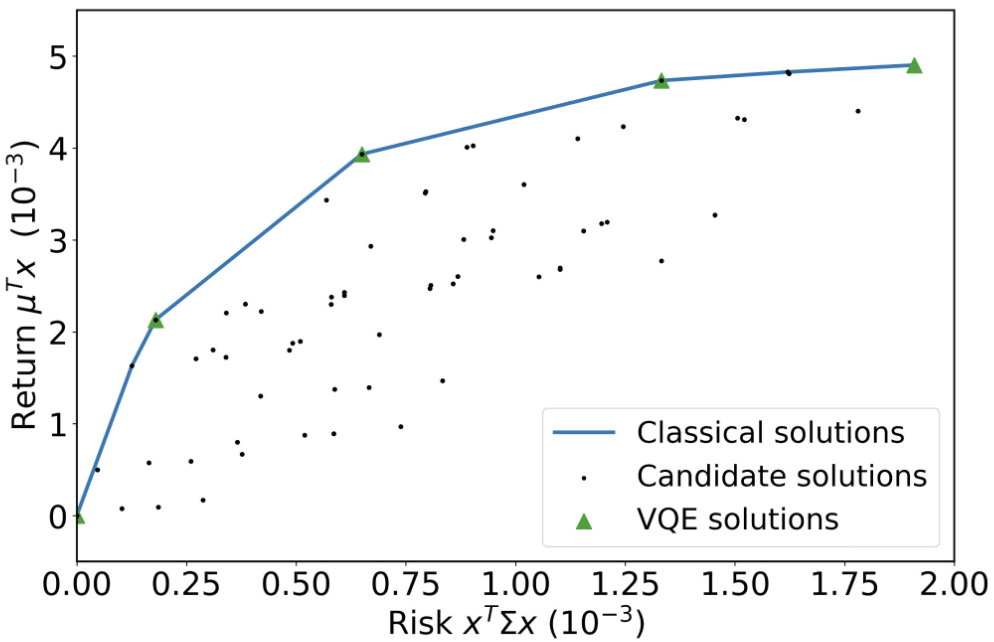
\includegraphics[width=0.8\linewidth]{EfficientFrontier_VQE.png}
    \caption{Beispiel einer Efficient Frontier in der Portfolio-Optimierung (simuliertes 6-Asset-Portfolio). Die blaue Kurve zeigt die optimale Risiko-Rendite-Kurve (klassische Exhaustivsuche), die grünen Dreiecke markieren Lösungen des Quantum-VQE-Algorithmus. Man sieht, dass die Quantenlösungen die Effizienzgrenze eng nachzeichnen (Rendite $\mu^T x$ und Risiko $x^T \Sigma x$ sind in willkürlichen Einheiten). \cite[Abb. 8]{egger_quantum_2020}}
    \label{fig:efficient_frontier_vqe}
\end{figure}


Abb. \ref{fig:efficient_frontier_vqe} illustriert, dass bereits heutige gate-basierte Quantenalgorithmen wie der VQE in der Lage sind, für kleine Portfolios (hier ein simuliertes 6-Asset-Portfolio) ähnlich effiziente Lösungen wie klassische Exhaustivsuche zu erzeugen. Die grünen Dreiecke zeigen, dass die vom VQE generierten Lösungen eng entlang der klassischen Efficient Frontier liegen. Dies verdeutlicht das Potenzial quantenbasierter Optimierung in Kombination mit VQE, insbesondere für risikoertragsbasierte Portfolioentscheidungen. Die zugrunde liegende Studie von Egger et al. (2020) demonstriert damit erfolgreich die prinzipielle Machbarkeit dieser Methode auf simulierten Quantencomputern. Einschränkungen bestehen jedoch weiterhin in Bezug auf Skalierbarkeit, da größere Portfolios tiefere Schaltkreise und längere Optimierung erfordern.
 
Gleichzeitig zeigen erste Studien jedoch, dass unter kontrollierten Bedingungen bereits vielversprechende Ergebnisse erzielt werden können. So testeten mehrere Arbeiten die Wirksamkeit von VQE-Pipelines. Die Ergebnisse lieferten, dass der VQE auf einem 5-Qubit-Gerät eine fast identische Lösung zum klassischen Optimum generieren konnte. Die Qualität der Lösung variierte jedoch mit der Qualität des Quantenchips. Größere und weniger von Rausch behaftete Geräte lieferten verbesserte Ergebnisse als kleinere. Somit schmälern Rauschen und die begrenzte Qubit-Zahlen zwar noch den Nutzen, obwohl die Algorithmen prinzipiell eine optimale Lösung bieten \cite{buonaiuto_best_2023}.
Der Einsatz von QAOA mit der Fixierung der Anzahl der enthaltenen Assets zeigte, dass die Anzahl benötigter Quantengatter und Messungen, die für mittlere Problemgrößen benötigt werden, die NISQ-Geräte an ihre Grenzen bringt. Für kleinere Portfolios konnten jedoch annähernd optimale Ergebnisse erzielt werden \cite{brandhofer_benchmarking_2022}.
 
Beide Ansätze QAOA/VQE glänzen in Ihrer Flexibilität. Es können leichter zusätzliche Nebenbedingungen eingebaut und dynamische Portfolio-Probleme formuliert werden. Nachteile spiegeln sich in der Limitation durch Rauschen und Dekohärenz wider, die ohne notwendige Fehlerkorrektur nicht behoben werden können. Aufgrund dieser Einschränkungen bleiben die Anwendungen der gate-basierten Ansätze noch auf rein simulierter Ebene oder auf kleinen Hardware-Experimenten beschränkt.

\subparagraph{Chancen und Herausforderungen}

Gate-basierte Algorithmen wie VQE bieten ein hohes Maß an Anpassungsfähigkeit für Portfoliooptimierungsprobleme, insbesondere im Umgang mit komplexen Nebenbedingungen. Erste Tests auf realer Hardware zeigen, dass bei kleinen Portfolios bereits Lösungen in Nähe des klassischen Optimums erzielt werden können \cite[S. 2–4]{buonaiuto_best_2023}. Dabei hängt die Qualität stark von den gewählten Hyperparametern und der verwendeten Hardware ab. Je größer und rauschärmer das Quantenchip, desto näher die Lösung an der klassischen Referenz. Allerdings bleiben signifikante Herausforderungen bestehen: Skalierungsprobleme, Rauschanfälligkeit und die Auswahl geeigneter Optimierer beeinflussen die Ergebnisse maßgeblich. Trotz des hohen Potenzials für künftige Verbesserungen ist ein praktischer Vorteil gegenüber klassischen Methoden bislang nicht eindeutig belegt.

\subsection{ Monte Carlo Simulation}

Die Bewertung von Anlagen und Portfolios bedingt eine enorme Komplexität durch die
unvollkommene Verteilung von Informationen auf Finanzmärkten. Entscheidungen über Risikostrategien, Bewertungen und Investitionen müssen häufig in Situationen getroffen werden, in denen wirtschaftliche Verläufe nicht direkt einsichtig sind. Hierbei greifen Marktteilnehmer auf Schätzungen, Wahrscheinlichkeiten und historische Daten zurück, um zukünftige Entwicklungen zu bewerten. 
\\
 Als grundlegendes Instrument wird in diesem Bereich die Monte-Carlo-Simulation in Betracht gezogen. Mithilfe der Monte-Carlo-Simulation können die Lösungen von analytisch komplexen und schwer lösbaren mathematischen Problemen geschätzt werden. Es nutzt also statistische Simulierung und Zufallsstichproben, um wiederholt verschiedene Szenarien eines Systems zu simulieren und Erwartungswerte oder Wahrscheinlichkeiten approximativ zu bestimmen.\cite{orus_quantum_2019}.
 
Typische Anwendungsfelder dieses stochastischen Ansatzes sind: Optionsbewertung (Pricing von Derivaten, deren Auszahlung vom zukünftigen Preisverlauf eines Basiswerts abhängt) und Risikobemessung (Berechnung des Value at Risk für ein Portfolio über einen Zeithorizont). Letzteres wird in Kapitel 4.3.3 näher beleuchtet \cite{orus_quantum_2019}. Sowohl die Optionsbewertung als auch die Risikobemessung stellen zentrale Aufgaben im Finanzwesen dar, bei denen zukünftige, stochastisch unsichere Größen quantifiziert werden müssen. Aufgrund der Komplexität moderner Finanzinstrumente und der hohen Dimensionalität der zugrunde liegenden Zufallsprozesse sind analytische Lösungen häufig nicht verfügbar. Die Monte-Carlo-Simulation dient in beiden Anwendungsfeldern als methodisches Fundament, um durch zufällige Stichproben komplexe Erwartungswerte oder Verteilungsquantile numerisch zu vergleichen. Damit bildet sie die Grundlage zahlreicher Bewertungs- und Risikomodelle in Praxis und Forschung.

\subsubsection*{Optionsbewertung}
Die Bewertung von Optionen erfordert häufig numerische Verfahren, da für viele Ausgestaltungen keine geschlossenen analytischen Lösungen existieren. Besonders bei komplexeren Derivaten wie asiatischen Optionen, Barrier-Optionen oder Portfolios von Optionen muss meist numerisch simuliert werden. Optionen stellen Finanzderivate dar, wobei ein Derivat ein Instrument ist, dessen Preisentwicklung von der Entwicklung einer oder mehrerer Anlagen abhängt. Das Monte-Carlo-Verfahren nutzt hierbei eine große Menge an Zufallspfad-Simulationen generiert für die relevanten Prozesse und errechnet aus den Auszahlungen oder Verlusten statistische Kennzahlen. Faktisch wird versucht, den „fairen“ Preis einer Option zu ermitteln. Dazu werden mögliche Pfade, die der Aktienkurs einnehmen könnte, bis zur Fälligkeit simuliert, für jeden Pfad die Auszahlung berechnet und gemittelt\cite{orus_quantum_2019}.
 
Damit die Verteilungsmerkmale in der geforderten Genauigkeit erfasst werden können, müssen ausreichend Pfade generiert werden. Das Gesetz der großen Zahlen bestimmt hierbei dass die Schätzung des Erwartungswertes mit der Anzahl N der simulierten Pfade ungefähr mit $1/\sqrt{N}$ konvergiert. Diese Konvergenz ist verhältnismäßig gering. Um die Genauigkeit, um genau eine Einheit zu verbessern, muss die Zahl der Simulationsläufe um das Vierfache erhöht werden. Dadurch steigt die Zahl der Pfade schnell auf eine Millionen oder Milliarden Höhe an.
In der Praxis ist genau das eins der größten Probleme. Komplexe Berechnungen von zum Beispiel Kreditrisiko-Simulationen von Hunderten von Banken und Unternehmen können Tage dauern. Trotz der stetigen Parallelisierung stoßen herkömmliche Methoden aufgrund der Rechenzeit und Kosten an Ihre Grenzen \cite{orus_quantum_2019}.

\subsubsection*{Quantenbasierte Methoden zur Optionsbewertung}
Durch methodische Erweiterungen, wie der Quantum Amplitude Estimation (QAE) können Prozesse der klassischen Monte-Carlo Simulation beschleunigt werden. Bei dem Fall der Optionsbewertung, müssen Wahrscheinlichkeitsverteilungen über zukünftige Assetpreise quantenmechanisch kodiert werden. Diesbezüglich wird QAE angewendet, um effiziente Schätzungen des Erwartungswertes, also die Bestimmung des “fairen” Optionspreises, zu gewährleisten. Im Vergleich zur klassischen Monte-Carlo-Methode, die für eine Zielgenauigkeit von $\varepsilon$ etwa $O(1/\varepsilon^2)$ Stichproben benötigt, minimiert QAE diesen Aufwand auf $O(1/\varepsilon)$. Praktisch bedeutet das, dass statt einer Million klassischer Proben rund 1000 Quantenproben ausreichen bei gleichbleibender Akkuratesse \cite{Brassard/Lomonaco+Brandt; Montanaro, 2015}.

In ersten Bewertungs-Workflows wurde dieser theoretische Ansatz bereits auf realer Quantenhardware getestet und demonstriert. Es wurden verschieden Optionsarten mithilfe passender Quantenschaltungen modelliert und darauf folgend mit Maximum-Likelihood-Amplitude-Estimation (MLAE) bewertet. Dieses Verfahren ist vorteilhafter als das klassische QAE, da es durch eine flachere Schaltung besser für die NISQ-Geräte geeignet ist. NISQ-Geräte (Noisy Intermediate-Scale Quantum) sind gegenwärtige Quantencomputer mit einer begrenzten Anzahl von Qubits und ohne vollständige Fehlerkorrektur, die bereits erste praktische Anwendungen ermöglichen, jedoch noch anfällig für Störungen und Skalierungsprobleme sind \cite{stamatopoulos_option_2020}.

Fehler können durch Kalibrierung von Zwei-Qubit-Gattern gedämpft werden, wodurch bereits aus Drei-Qubit-Schaltungen valide Optionspreise extrahiert werden konnten. Zentrale praktische Hindernisse bleiben jedoch bestehen. Besonders das effiziente Laden von Datenquellen und klassischen Wahrscheinlichkeitsverteilungen auf Quantenhardware stellt sich als kompliziert heraus. Um diese Marktszenarien, wie Asset-Preise, auf Quantencomputern zu verarbeiten, müssen die Daten in einen entsprechenden Quantenzustand überführt werden. Hiefür benötigen die klassischen Verfahren einen exponentiell steigenden Ressourcenaufwand von $O(2^n)$. Eine Lösung bietet Quantum Generative Adversial Networks (qGans), die aus den klassischen Marktdaten die passenden Wahrscheinlichkeitsverteilungen erlernt und anschließend als polynomieller Komplexität als Quantenzustand bereitstellt \cite{zoufal_quantum_2019}.

Zusammenfassend wird deutlich, dass QAE in Kombination mit verfahren wie MLAE, iterativen QAE oder variationalen Ansätzen zu einer Beschleunigung klassischer Monte-Carlo-Simulationen führt. In Verbindung mit effizienten Datenlagern wie qGANs rückt der Einsatz solcher Verfahren auf realer Quantenhardware in greifbare Nähe.

\subparagraph{Chancen und Herausforderungen}

Die Anwendung quantenmechanischer Verfahren zur Optionsbewertung, etwa durch Quantum Amplitude Estimation (QAE) oder Maximum-Likelihood-Amplitude-Estimation (MLAE), verspricht signifikante Rechenzeitvorteile gegenüber klassischen Monte-Carlo-Simulationen. In ersten Experimenten konnten realistische Optionspreise bereits aus wenigen Qubits extrahiert werden \cite[S. 4–6]{stamatopoulos_option_2020}, was das Potenzial für eine breitere Nutzung unterstreicht. Gleichzeitig bestehen technische Hürden: Insbesondere das effiziente Laden klassischer Wahrscheinlichkeitsverteilungen in Quantenregister ist rechenintensiv. Quantum Generative Adversarial Networks (qGANs) bieten hier einen vielversprechenden Ansatz zur effizienten Quantenzustandspräparation \cite[S. 1–3]{zoufal_quantum_2019}. Die hohe Variabilität exotischer Auszahlungsstrukturen und die Unsicherheit bei Modellkalibrierungen bleiben jedoch praktische Herausforderungen.

\subsection{Risikobemessung und Value at Risk}

Eine der zentralen Herausforderungen im modernen Finanzwesen ist die Risikobemessung. Um drohende Verluste rechtzeitig zu erkennen und gezielt Gegenmaßnahmen zu ergreifen, sind Banken, Investoren und andere Marktteilnehmer in einem hoch volatilen Marktumfeld darauf angewiesen, Risiken genau zu quantifizieren und zuverlässig einschätzen zu können. 
Auch in der Risikobemessung stellt die Monte-Carlo-Simulation ein zentrales Werkzeug dar, insbesondere zur Schätzung von Risikokennzahlen wie dem Value at Risk (VaR) oder dem Conditional Value at Risk (CVaR), die auf der Analyse stochastischer Verlustverteilungen basieren. Der VaR ist ein anerkanntes und gängiges Instrument zur Quantifizierung von Risiko und zeigt den maximalen Verlust an, den ein Portfolio oder eine einzelne Anlageposition innerhalb eines bestimmten Zeitraums und mit einer festgelegten Vertrauens-Wahrscheinlichkeit (in der Regel 95\,\% oder 99\,\%) nicht überschreiten wird \cite{springer2025, plos2024}. 
Für Finanzinstitutionen ist der VaR nicht nur methodisch relevant, sondern auch regulatorisch von hoher Bedeutung. Finanzinstitute wie Banken, Versicherungen und Investmentfonds sind gesetzlich verpflichtet, Marktrisiken und Kreditrisiken regelmäßig zu quantifizieren, um ausreichende Kapitalpuffer zu erzeugen. Die Risikokennzahlen dienen darüber hinaus intern der Begrenzung von Handelspositionen, etwa durch tägliche VaR-Limits für einzelne Portfolios oder Trader. Auch in der langfristigen Risikosteuerung, etwa bei Pensionskassen oder Versicherungen, sind VaR und CVaR zentrale Steuerungsgrößen, um sicherzustellen, dass finanzielle Verpflichtungen auch unter Stressszenarien eingehalten werden können \cite{Orús et al., 2019}.
Trotz seiner weiten Verbreitung ist der VaR nicht frei von Kritik. Insbesondere die fehlende Subadditivität kann bei der Aggregation von Risiken zu fehlerhaften Einschätzungen führen. Der CVaR wurde als kohärentes Risikomaß eingeführt, um auch die Schwere der Verluste im Extrembereich zu erfassen und gilt in vielen Anwendungen als präzisere Alternative \cite{orus_quantum_2019}.In der Praxis lassen sich VaR und CVaR nur in einfachen Fällen analytisch berechnen. Komplexe Portfolios mit nicht-normalverteilten Erträgen oder Derivatebestandteilen erfordern numerische Verfahren. Die Monte-Carlo-Simulation ist hier besonders geeignet, um aus vielen simulierten Szenarien empirische Verlustverteilungen abzuleiten und daraus die relevanten Quantile zu bestimmen \cite{Zoufal et al., 2019}.

Die Monte-Carlo-Simulation gilt zwar als Standardverfahren zur Schätzung komplexer Verlustverteilungen, stößt jedoch bei steigender Modellkomplexität schnell an ihre Grenzen. Mit zunehmender Anzahl an Risikofaktoren, Anlageklassen oder eingebetteten Derivaten steigt der Rechenaufwand drastisch an. Insbesondere die Ermittlung von Extremrisiken wie dem 99{,}9\,\%\,VaR erfordert Millionen von Simulationsläufen, was selbst auf leistungsstarken Rechnern mit erheblichen Laufzeiten verbunden ist. Für verschachtelte Portfolios kommt es häufig zu sogenannten Nested-Monte-Carlo-Strukturen, bei denen für jedes Szenario zusätzliche Bewertungen durchgeführt werden müssen. Die resultierende Rechenzeit verhindert eine laufende Risikobewertung in kurzen Intervallen und erschwert eine schnelle Reaktion in volatilen Marktphasen \cite{bouland_prospects_2020, orus_quantum_2019}


\subsubsection*{Quantenbasierte Methoden zur Risikobemessung}

In Anbetracht der rechentechnischen Hürden klassischer Risikosimulationen rückt Quantum Computing als vielversprechender Lösungsansatz zunehmend in den Fokus. Besonders relevant ist hierbei der Quantum-Amplitude-Estimation-Algorithmus (QAE), der bei der Berechnung stochastischer Erwartungswerte eine quadratische Beschleunigung gegenüber klassischen Monte-Carlo-Verfahren ermöglicht \cite{quantumjournal2020, rebentrost_quantum_2018}. Der Vorteil des QAE besteht darin, dass weniger Simulationsläufe benötigt werden, um eine Zielgenauigkeit $\varepsilon$ zu erreichen, da die Komplexität von $O(1/\varepsilon^2)$ auf $O(1/\varepsilon)$ reduziert wird \cite{martin2022}. Dies ist besonders relevant bei der Schätzung seltener Ereignisse wie dem 99{,}9\,\%-VaR, bei dem klassisch Millionen bis Milliarden Pfade erforderlich wären.

Zur Anwendung von QAE im Risikokontext wird ein Orakel-Operator entworfen, der für ein bestimmtes Verlustniveau $x$ anzeigt, ob der simulierte Portfolioverlust dieses Niveau überschreitet. Mittels QAE lässt sich dann die Wahrscheinlichkeit $P(\text{Verlust} > x)$ effizient bestimmen. Durch Variation von $x$ kann so derjenige Schwellenwert ermittelt werden, für den die Überschreitungswahrscheinlichkeit einem definierten Konfidenzniveau entspricht, was exakt der Definition des Value at Risk entspricht. Analog dazu lässt sich auch der Conditional Value at Risk berechnen, indem ein modifizierter Schaltkreis verwendet wird, der den durchschnittlichen Verlust im Überschreitungsfall quantifiziert \cite{orus_quantum_2019, egger_quantum_2020}.

Die Umsetzung dieser quantenmechanischen Verfahren erfordert jedoch eine geeignete Repräsentation der Verlustverteilung auf dem Quantencomputer. Dazu müssen komplexe stochastische Prozesse, wie sie etwa durch Marktrisiken und Korrelationen zwischen verschiedenen Risikofaktoren entstehen, in einem Quantenzustand abgebildet werden. Eine direkte Kodierung solcher Verteilungen auf Quantenhardware ist jedoch exponentiell aufwendig, weshalb quantum-native Methoden wie Quantum Generative Adversarial Networks (qGANs) eingesetzt werden. Diese Netzwerke sind in der Lage, aus realen Marktdaten eine Zielverteilung zu lernen und diese in polynomieller Komplexität als Quantenzustand bereitzustellen \cite{zoufal_quantum_2019}. Kombiniert mit vereinfachten QAE-Varianten wie dem Maximum-Likelihood-Amplitude-Estimation (MLAE), die flachere Quantenschaltkreise erzeugen, können solche Verfahren auch auf heutiger NISQ-Hardware eingesetzt werden \cite{stamatopoulos_option_2020}.

Erste Proof-of-Concept-Studien zeigen, dass quantenbasierte Risikomessung prinzipiell umsetzbar ist. In einer wegweisenden Arbeit demonstrierten Woerner und Egger die Berechnung des VaR für ein vereinfachtes Anleiheportfolio mit Hilfe eines IBM-Q-Prozessors. Trotz der Beschränkung auf wenige Qubits konnten valide Resultate erzeugt werden, die die klassische Berechnung reproduzierten \cite{egger_quantum_2020}. Aufbauend darauf wurden in weiteren Studien der potenzielle Ressourcenbedarf für realistische Risikoszenarien analysiert. Diese Arbeiten kommen zu dem Ergebnis, dass für große Portfolios mit vielen Risikofaktoren und hohen Konfidenzniveaus fehlerkorrigierte Quantencomputer mit deutlich größerer Qubit-Anzahl erforderlich wären. Gleichzeitig wurden aber auch Ansätze zur Reduktion der Komplexität untersucht, etwa durch grobe Vorabschätzungen mittels klassischer Simulation oder durch analytische Näherungen innerhalb des quantenbasierten Modells \cite{martin2022}.

Auch in der Finanzindustrie wächst das Interesse an quantenbasierter Risikomodellierung. Verschiedene Banken, Technologieunternehmen und Start-ups forschen an hybriden Architekturen, bei denen klassische und Quantencomputer kombiniert werden. Ziel ist es, einzelne Komponenten wie die Quantilschätzung gezielt zu beschleunigen und so tägliche Risikoberichte effizienter zu gestalten. Langfristig wird angestrebt, komplexe Verlustverteilungen nahezu in Echtzeit zu analysieren und damit ein neues Niveau an Präzision und Reaktionsgeschwindigkeit im Risikomanagement zu erreichen \cite{orus_quantum_2019, bouland_prospects_2020}.

Insgesamt zeigt sich, dass quantenbasierte Methoden wie QAE das Potenzial haben, bestehende Grenzen klassischer Risikoberechnung deutlich zu verschieben. Zwar steht die praktische Umsetzung noch am Anfang, doch bereits heute belegen erste experimentelle Studien den theoretischen Vorteil und die prinzipielle Machbarkeit. Mit zunehmender Reife der Quantenhardware sowie verbesserter Datenkodierung und Fehlerkorrektur könnten quantenmechanische Simulationen zu einem festen Bestandteil moderner Finanzanalyse werden.

\subparagraph{Chancen und Herausforderungen}

Quantengestützte Risikomodellierung verspricht eine signifikante Beschleunigung bei der Schätzung von Value at Risk und Conditional Value at Risk, insbesondere in Szenarien mit hohen Konfidenzniveaus und komplexer Portfoliostruktur. QAE reduziert die erforderliche Anzahl an Simulationsläufen drastisch und ermöglicht präzisere Risikoberichte bei geringerem Rechenaufwand \cite[S. 6–7]{orus_quantum_2019}. Gleichzeitig sind praktische Anwendungen noch limitiert: Das Laden komplexer Verlustverteilungen ist technisch aufwendig, und aktuelle NISQ-Geräte stoßen bei umfangreichen Risikomodellen rasch an Grenzen. Auch klassische Monte-Carlo-Verfahren leiden unter ähnlichen Problemen, insbesondere bei Konvergenzgeschwindigkeit und Modellrisiken \cite[S. 1–2]{MonteCarloSim2023}. Quantenverfahren zeigen daher bislang insbesondere bei strukturierten, datengetriebenen Subproblemen einen Vorteil.

\begin{table}[!htbp]
\centering
\renewcommand{\arraystretch}{1.5}
\begin{tabular}{|p{0.25\linewidth}|p{0.23\linewidth}|p{0.23\linewidth}|p{0.23\linewidth}|}
\hline
\textbf{Anwendungsfeld} & \textbf{Problem} & \textbf{Quantenlösung} & \textbf{Technologie(n)} \\
\hline
\textbf{Portfolio-optimierung} & 
Kombinatorische Auswahl aus Assets mit Budget/Risiko & 
Binäre Optimierung mit Energie-Minimum-Suche & 
\begin{minipage}[t]{\linewidth}
\begin{itemize}[leftmargin=*,noitemsep]
  \item Quantum Annealing (D-Wave)
  \item QAOA/VQE (gate-basiert)
\end{itemize}
\end{minipage} \\
\hline
\textbf{Optionsbewertung} & 
Erwartungswert der Auszahlung über viele Pfade & 
Schätzung des Mittelwerts über quantisierte Wahrscheinlichkeiten & 
\begin{minipage}[t]{\linewidth}
\begin{itemize}[leftmargin=*,noitemsep]
  \item QAE
  \item MLAE (NISQ-kompatibel)
\end{itemize}
\end{minipage} \\
\hline
\textbf{Risikomessung (VaR/CVaR)} & 
Quantile aus Verlustverteilung (extreme Szenarien) & 
Amplitude-Schätzung von Überschreitungswahrscheinlichkeit & 
\begin{minipage}[t]{\linewidth}
\begin{itemize}[leftmargin=*,noitemsep]
  \item QAE
  \item QAE + qGANs
\end{itemize}
\end{minipage} \\
\hline
\end{tabular}
\caption{Übersicht der Anwendungsfelder und Quantenlösungen im Finanzbereich}
\label{tab:qc_overview}
\end{table}






\section{Top Technologien und Algorithmen}

Im vorangegangenen Kapitel wurden drei zentrale Anwendungsfelder vorgestellt, in denen quantenbasierte Verfahren im Finanzwesen potenzielle Vorteile gegenüber klassischen Methoden aufweisen. In all diesen Bereichen werden spezifische Quantenalgorithmen verwendet, die auf unterschiedlichen technologischen Prinzipien beruhen. Das Verständnis dieser Verfahren ist ausschlaggebend, um ihr Potenzial, ihre Grenzen und ihre technische Realisierbarkeit richtig einzuordnen.

Mit der zunehmenden Komplexität moderner Finanzmodelle und der stetig wachsenden Menge verfügbarer Daten stoßen klassische Rechenverfahren an fundamentale Grenzen. Besonders bei Aufgaben, die eine hohe kombinatorische Tiefe oder stochastische Genauigkeit erfordern, wie etwa die Bewertung von komplexen Derivaten oder die Simulation von extremen Risiken, geraten klassische Architekturen an ihre Grenzen \cite{plos2024, bouland_prospects_2020}.

In solchen Szenarien versprechen Quantencomputer neue Lösungsansätze. Sie nutzen grundlegende Eigenschaften der Quantenmechanik wie Superposition und Verschränkung, um bestimmte Klassen von Problemen effizienter zu bearbeiten. Während klassische Computer Informationen in Form von Bits (0 oder 1) verarbeiten, ermöglichen Quantenbits (Qubits) die gleichzeitige Darstellung und Verarbeitung vieler Zustände. Das kann in spezifischen Fällen zu einer erheblichen Beschleunigung oder einer höheren Ergebnisgüte führen \cite{orus_quantum_2019, bouland_prospects_2020, martin2022}.

Im Rahmen der zuvor beschriebenen Anwendungen wurden bereits konkrete Quantenansätze eingeführt. Dieses Kapitel widmet sich nun vertiefend den zugrunde liegenden Technologien und Algorithmen. Ziel ist es, ihre Funktionsweise, ihre strukturellen Voraussetzungen und ihre Eignung für verschiedene Problemstellungen im Finanzbereich systematisch darzustellen.

Zu den derzeit zentralen quantenbasierten Methoden im Finanzkontext gehören:

\begin{itemize}
  \item Quantum Annealing (QA)
  \item Gate-basierte Algorithmen
    \begin{itemize}
      \item Quantum Approximate Optimization Algorithm (QAOA)
      \item Variational Quantum Eigensolver und verwandte Variationsansätze (VQE, VQA)
    \end{itemize}
  \item Quantum Amplitude Estimation (QAE)
\end{itemize}

Die folgenden Abschnitte analysieren diese Technologien aus technischer Perspektive. Sie zeigen, welche Stärken und Schwächen mit den jeweiligen Ansätzen verbunden sind und welche praktischen Voraussetzungen für deren erfolgreichen Einsatz im Finanzwesen erfüllt sein müssen.

\subsection{Quantum Annealing (QA)}

Quantum Annealing ist ein quantenmechanisches Optimierungsverfahren, das für kombinatorische Probleme eingesetzt wird. Es wird insbesondere in der Portfoliooptimierung verwendet, kommt aber auch in Bereichen wie Arbitrage-Erkennung, Kreditrisikoanalyse und Supply-Chain-Prozessen zum Einsatz \cite{orus_quantum_2019, mugel_dynamic_2022}.

Technologisch basiert Quantum Annealing auf dem adiabatischen Prinzip. Dabei wird das Quantensystem aus einem bekannten Anfangszustand (Anfangshamiltonian) langsam in den Problemzustand überführt. Solange dieser Vorgang ausreichend langsam erfolgt, bleibt das System im energetisch niedrigsten Zustand, der die optimale Lösung enthält \cite{Orus2019}. Das zugrunde liegende Problem muss dafür in ein Quadratic Unconstrained Binary Optimization (QUBO)-Modell oder ein Ising-Modell transformiert werden. Die binären Entscheidungsvariablen repräsentieren Investitionsentscheidungen, die Wechselwirkungen codieren Rendite, Risiko und Constraints. Auf der Hardware wird jeder Qubit einer Variablen zugewiesen, und Kopplungen entsprechen den Interaktionen der Modellstruktur. Während des Annealing-Prozesses wird das System kontrolliert „heruntergekühlt“, bis es in einem möglichst optimalen Zustand verharrt \cite{mugel_dynamic_2022, Rosenberg2016}. Diese Umsetzung ermöglicht eine praxisnahe Anwendung bei strukturierten Finanzproblemen, auch wenn die gegenwärtigen Systeme noch Einschränkungen in der Skalierbarkeit aufweisen \cite{sakuler_real-world_2025}.

Ein großer Vorteil von Quantum Annealing ist die effiziente Lösung diskreter Optimierungsprobleme. Es kann auf spezieller Hardware wie dem D-Wave-System implementiert werden, die physikalisch auf QUBO-Probleme ausgelegt ist. Durch quantenmechanisches Tunneling können lokale Minima überwunden und Lösungen schneller gefunden werden. Weitere Vorteile sind die gute Konvergenz bei kleinen bis mittelgroßen Instanzen und der natürliche Hardwarebezug \cite{mugel_dynamic_2022, sakuler_real-world_2025}. Zu den Nachteilen zählen die beschränkte Skalierbarkeit auf große Problemgrößen, die begrenzte Qubit-Konnektivität und die schwierige Abbildung komplexer Nebenbedingungen \cite{sakuler_real-world_2025}.

\subsection{Gate-basierte Ansätze (QAOA und VQE)}

Gate-basierte Quantencomputer arbeiten mit Schaltkreisen. Auf diesen Systemen können Variationsalgorithmen implementiert werden, die Optimierungsprobleme lösen. Die zwei bekanntesten Methoden sind hierbei Quantum Approximate Optimization Algorithm (QAOA) und Variational Quantum Eigensolver (VQE). In beiden Methoden kommt ein parametrischer Quantenschaltkreis zum Einsatz, dessen Parameter iterativ von einem klassischen
Optimierer so eingestellt werden, dass das gemessene Ausgabe-Stadium die Zielfunktion minimiert. Für die Portfoliooptimierung muss zuerst das eigentliche Problem abgeleitet und in einen Hamiltonoperator übersetzt werden \cite{buonaiuto_best_2023, brandhofer_benchmarking_2022}.
 
\subsubsection*{Quantum Approximate Optimization Algorithm (QAOA)}
Für den Quantum Approximate Optimization Algorithm (QAOA) Ansatz muss durch die Umwandlung in ein Ising-Modell zunächst das Optimierungsproblem binär formuliert werden. Dieses Modell bildet mit Wechselwirkungsparametern zwischen den Qubits das Ertrags-Risiko-Profil des Portfolios ab \cite{brandhofer_benchmarking_2022}.
Der QAO-Algorythmus verwendet abwechselnd zwei Arten von Gate-Operationen. Eine Operation auf dem Problem Hamiltonian basierenden Phasenschicht und eine auf einer Mixer-Hamiltonian Rotationsschicht. ­Die Anzahl der Alternierungen zwischen Misch- und Phasen-Gates ist bestimmt durch die Tiefe. Ziel ist es, die Messwahrscheinlichkeit für eine optimale Lösung zu verbessern. In der Studie von Brandhofer et al. (2023), zeigen die Autoren, dass der Einsatz von diesen spezialisierten Mixern, die Güte und die Umsetzbarkeit der Lösung deutlich verbessert.

\subsubsection*{Variational Quantum Eigensolver (VQE)}
Der Variational Quantum Eigensolver (VQE) verfolgt zwar vom grundsatz her ein ähnliches Ziel, verwendet jedoch einen anderen Ansatz. Statt des festgelegten Schematas bei QAOA, ist die Wahl des Schaltkreises beliebig und mit festen Parametern versehen. Der Erwartungswert des Problem-Hamiltonians wird durch wiederholtes Messen geschätzt, und ein klassischer Optimierer passt die Parameter an, um den Energieerwartungswert zu minimieren. Die Ansätze können beispielsweise Hardware-effizient oder Problem-spezifisch sein \cite{brandhofer_benchmarking_2022}.

\subsection{Quantum Amplitude Estimation (QAE)}

Quantum Amplitude Estimation (QAE) ist ein quantenmechanischer Algorithmus, der von Brassard et al. entwickelt wurde und sich besonders für die Beschleunigung Monte-Carlo-basierter Verfahren eignet \cite{quantumjournal2020}. In der Finanzwelt wird QAE zur Bewertung komplexer Finanzinstrumente wie Optionen sowie zur Modellierung von Kreditrisiken und stochastischen Prozessen verwendet \cite{rebentrost2018, egger2020}.

Technologisch kombiniert QAE Quantenamplitudeninterferenz mit Messstrategien, um Erwartungswerte effizienter zu schätzen als klassische Monte-Carlo-Algorithmen. Während herkömmliche Verfahren $O(1/\varepsilon^2)$ Stichproben zur Erreichung einer Genauigkeit $\varepsilon$ benötigen, reduziert QAE diesen Aufwand auf $O(1/\varepsilon)$ \cite{quantumjournal2020, martin2022}. Die zugrunde liegende Quantenroutine nutzt dabei quantenmechanische Effekte wie Superposition und Interferenz, um Wahrscheinlichkeiten zu verstärken, die zur Zielausgabe führen. Anwendungen beinhalten insbesondere die Bewertung pfadabhängiger Optionen, Value-at-Risk-Simulationen sowie generelle Risiko- und Bewertungsmodelle, bei denen große Stichprobenmengen erforderlich sind \cite{orus_quantum_2019, rebentrost2018}.

Ein zentraler Vorteil von QAE liegt in der quadratischen Beschleunigung gegenüber klassischen Verfahren, was zu erheblichen Effizienzgewinnen bei der Bewertung komplexer Modelle führen kann \cite{rebentrost2018}. Zudem ermöglicht QAE die Verarbeitung realitätsnäherer Modelle, die mit klassischen Methoden oft rechnerisch unpraktikabel wären.

Zu den Nachteilen gehört vor allem der aktuelle Stand der Quantenhardware. Begrenzte Qubit-Anzahlen, kurze Kohärenzzeiten und Messfehler erschweren die skalierbare Umsetzung in der Praxis \cite{bouland_prospects_2020, martin2022}. Auch erfordert QAE oft tiefe Quantenschaltkreise, was den Einsatz auf heutigen NISQ-Geräten (Noisy Intermediate-Scale Quantum) einschränkt.

Trotz dieser Herausforderungen arbeiten Industrie und Forschung an der praktischen Umsetzung. Besonders Partnerschaften zwischen Banken wie JPMorgan und Technologieunternehmen wie IBM zeigen, dass der Einsatz von QAE in der Finanzpraxis in naher Zukunft realistisch sein könnte \cite{egger2020}.

\section{Wichtige Unternehmen und Akteure und Ihre Zukunftsprojekte}
Der Fortschritt im Quantencomputing für Finanzanwendungen wird wesentlich von der engen Vernetzung führender Technologieunternehmen, Finanzinstitute und Forschungsinitiativen geprägt. Einige Akteure entwickeln Hardware und Plattformen, andere arbeiten direkt an Algorithmen oder Pilotprojekten. Im Folgenden werden die wichtigsten Akteure vorgestellt und ihre Projekte zugeordnet.

\subsection{IBM und JPMorgan: Technologie trifft Anwendung}

IBM zählt zu den globalen Vorreitern im Bereich Quantencomputing. Über die Cloudplattform IBM Quantum stellt das Unternehmen supraleitende Quantenprozessoren und entsprechende Entwicklungsumgebungen bereit. Partnerunternehmen können dort eigene Algorithmen entwickeln, testen und auf realer Quantenhardware ausführen. Im Finanzsektor nimmt IBM eine zentrale Rolle ein, indem es nicht nur Infrastruktur anbietet, sondern auch aktiv an der Entwicklung domänenspezifischer Quantenlösungen mitwirkt.
Ein bedeutender Kooperationspartner ist JPMorgan Chase, eine der ersten Banken, die strategisch auf Quantencomputing setzen. Im Rahmen der IBM-Quantum-Partnerschaft forscht JPMorgan an Anwendungen zur Bewertung komplexer Finanzinstrumente und zur Risikomodellierung (Moody’s, 2024). Besonders im Fokus steht die Quantum Amplitude Estimation (QAE), ein Algorithmus, der klassische Monte-Carlo-Simulationen deutlich effizienter gestaltet. Durch QAE lässt sich der Rechenaufwand zur Berechnung von Erwartungswerten signifikant verringern, was für Finanzanwendungen wie die Derivatebewertung oder die Berechnung des Value at Risk (VaR) besonders relevant ist (Larsson & Oosterlee, 2019; Schuld, 2020).
Ein weiteres gemeinsames Forschungsfeld ist die Quantum Random Number Generation (QRNG), bei der echte Zufallszahlen aus quantenphysikalischen Effekten gewonnen werden. Solche Zufallszahlen können klassische Pseudozufallsverfahren ersetzen und liefern robustere Ergebnisse für Simulationen und stochastische Modelle (Schuld, 2020). Die Kombination aus verbesserter Genauigkeit und höherer Rechengeschwindigkeit macht quantengestützte Verfahren für den Finanzsektor besonders vielversprechend.
Die Kooperation zwischen IBM und JPMorgan steht exemplarisch für eine enge Verzahnung von technologischer Innovation und praktischer Finanzanwendung. IBM stellt die Hardware und Softwareplattform bereit, während JPMorgan konkrete Anwendungsfälle identifiziert und validiert. Dadurch entsteht ein messbarer Erkenntnisgewinn für beide Seiten und ein reales Testfeld für die Leistungsfähigkeit aktueller Quantenalgorithmen im Finanzkontext (Moody’s, 2024).

\subsection{Microsoft und Alphabet: Infrastruktur ohne konkreten Finanzfokus}

Microsoft und Alphabet zählen zu den technologisch führenden Unternehmen im Bereich des Quantencomputings. Beide Konzerne investieren umfangreich in Forschung und Entwicklung und betreiben eigene Quantenplattformen, die den Zugang zu verschiedenen Hardwarearchitekturen ermöglichen. Im Gegensatz zu IBM fokussieren sich Microsoft und Alphabet bislang jedoch primär auf die infrastrukturelle Ebene. Konkrete, öffentlich dokumentierte Finanzanwendungen oder Partnerschaften mit Banken sind derzeit nicht bekannt.
Microsoft verfolgt mit der Plattform Azure Quantum einen Multi-Backend-Ansatz. Nutzer können über eine einheitliche Cloud-Umgebung auf verschiedene Quantenprozessoren zugreifen, darunter Anbieter wie IonQ, Quantinuum und Rigetti. Die Plattform richtet sich an Entwickler, Forschungseinrichtungen und Unternehmen, die eigene Quantenanwendungen testen oder simulieren möchten. Azure Quantum stellt damit eine flexible und leistungsstarke Infrastruktur zur Verfügung, die theoretisch auch für Finanzanwendungen geeignet ist. Bisher liegen jedoch keine spezifischen Kooperationen mit Finanzinstituten vor, in denen Microsoft aktiv quantenbasierte Lösungen für Risikoanalyse, Portfoliooptimierung oder Simulation mitgestaltet hätte (Microsoft Azure Quantum, 2024).
Alphabet verfolgt mit dem Quantum AI Lab einen stärker forschungsgetriebenen Ansatz. Der Fokus liegt auf der Weiterentwicklung supraleitender Quantenprozessoren sowie auf algorithmischen Innovationen, etwa im Bereich des maschinellen Lernens. Im Jahr 2019 erreichte Alphabet mit einem experimentellen Quantenprozessor einen wichtigen Meilenstein: die Demonstration der sogenannten Quantenvorherrschaft. Dabei wurde eine Aufgabe gelöst, die auf klassischen Computern kaum noch effizient berechnet werden kann (Arute et al., 2019). Trotz dieses Fortschritts beschränken sich die Aktivitäten von Alphabet bislang auf die Grundlagenforschung. Finanzanwendungen oder Kooperationen mit Banken wurden bisher nicht veröffentlicht (Google Quantum AI, 2024).
Sowohl Microsoft als auch Alphabet spielen eine zentrale Rolle beim Aufbau eines globalen Quantenökosystems. Ihre Plattformen tragen dazu bei, eine technologische Grundlage zu schaffen, auf der verschiedenste Branchen eigene Use Cases entwickeln können. Für den Finanzsektor bieten beide Unternehmen damit eine potenziell wertvolle Infrastruktur. Im Unterschied zu IBM engagieren sie sich bisher jedoch nicht direkt in der Entwicklung oder Validierung quantenspezifischer Anwendungen für finanzwirtschaftliche Problemstellungen.

\subsection{Europäische Perspektive: NEASQC und interdisziplinäre Zusammenarbeit}
Während große US-amerikanische Technologieunternehmen den Markt für Quantencomputing dominieren, verfolgt die Europäische Union mit gezielten Förder-programmen das Ziel, eigene Anwendungen für die NISQ-Ära zu entwickeln und gleichzeitig ihre technologische Souveränität zu stärken. Ein zentrales Vorhaben in diesem Kontext ist das Forschungsprojekt NEASQC (Next Applications of Quantum Computing), das im Rahmen des Horizon-2020-Programms der EU gefördert wird.
NEASQC bringt ein interdisziplinäres Konsortium aus Forschungseinrichtungen, Technologieunternehmen und Industriepartnern zusammen. Zu den beteiligten Organisationen gehören unter anderem Atos, das französische Forschungsinstitut CEA sowie als einziger Finanzakteur die Großbank HSBC. Ziel des Projekts ist es, praxistaugliche Algorithmen für aktuelle Quantenhardware zu entwickeln und anwendungsnah zu testen. Der Fokus liegt dabei auf sogenannten NISQ-Geräten, also Quantencomputern mit begrenzter Qubit-Anzahl und ohne vollständige Fehlerkorrektur (NEASQC, 2025).
Im Finanzbereich konzentriert sich NEASQC auf drei zentrale Anwendungsfelder: Monte-Carlo-Simulation, Portfolioanalyse und Hauptkomponentenanalyse (PCA). Dabei werden klassische Verfahren durch quantenmechanische Ansätze ersetzt oder ergänzt, etwa mithilfe von Quantum Amplitude Estimation, Quantum Machine Learning oder variationalen Algorithmen. In einem konkreten Anwendungsfall arbeitet HSBC gemeinsam mit Partnern an der Beschleunigung stochastischer Risikomodelle und der Entwicklung von Quantenschemata zur Optionsbewertung (Manzano et al., 2024; Zenodo, 2025).
Besonderes Gewicht liegt im Projekt auf der offenen Veröffentlichung von Ergebnissen und Tools. NEASQC verfolgt eine Open-Source-Strategie, bei der entwickelte Algorithmen und Testumgebungen für Dritte verfügbar gemacht werden, um Transparenz, Anschlussfähigkeit und Transfer in andere Anwendungsbereiche zu ermöglichen (NEASQC, 2025).
Das Projekt gilt als wichtiger Baustein der europäischen Quantenstrategie, da es nicht nur technische Entwicklungen fördert, sondern auch den Dialog zwischen Wissenschaft, Wirtschaft und öffentlicher Hand institutionalisiert. Für den Finanzsektor bietet NEASQC damit die Möglichkeit, die Anwendbarkeit quantenbasierter Methoden unter realen Bedingungen frühzeitig zu evaluieren und europaweit nutzbare Standards und Vorgehensweisen mitzugestalten (Finextra, 2020).

\section{Bewertung anhand der Kriterien}

Auf Basis der in diesem Kapitel analysierten Anwendungsfelder erfolgt im Folgenden eine vergleichende Bewertung der drei zentralen Einsatzbereiche von Quantencomputing im Finanzwesen: Portfoliooptimierung, Optionsbewertung und Risikomessung (Value at Risk / Conditional Value at Risk). Die Bewertung orientiert sich an fünf übergeordneten Kriterien: technologischer Reifegrad, wirtschaftliche Nutzbarkeit, gesellschaftlicher Nutzen, Forschungspotenzial sowie Risiken und ethische Implikationen.

Ziel dieser Gegenüberstellung ist es, die unterschiedlichen Entwicklungsstände, Chancen und Herausforderungen der betrachteten Anwendungsfelder systematisch einzuordnen. Dabei wird deutlich, in welchen Bereichen bereits erste praxisnahe Anwendungen existieren und wo insbesondere aus wissenschaftlicher Perspektive weiterführende Forschung notwendig ist, um das volle Potenzial quantenbasierter Methoden auszuschöpfen.



\begin{table}[!htbp]
\centering
\renewcommand{\arraystretch}{1.5}
\begin{tabular}{|p{0.25\linewidth}|p{0.23\linewidth}|p{0.23\linewidth}|p{0.23\linewidth}|}
\hline
\textbf{Kriterium} & \textbf{Portfoliooptimierung} & \textbf{Optionsbewertung} & \textbf{Risikobemessung (VaR/CVaR)} \\
\hline
Technologischer Reifegrad & mittel & niedrig & niedrig \\
\hline
Marktrelevanz & hoch & hoch & sehr hoch \\
\hline
Gesellschaftlicher Nutzen & mittel & mittel & hoch \\
\hline
Forschungspotenzial & hoch & sehr hoch & sehr hoch \\
\hline
Risiken und Ethik & gering & mittel & hoch \\
\hline
\end{tabular}
\caption{Bewertung der drei Hauptanwendungsfelder von Quantencomputing im Finanzwesen}
\label{tab:anwendungsbewertung}
\end{table}


\subsection*{Erläuterung der Bewertungskriterien}

Im Folgenden werden die fünf Bewertungskriterien der Tabelle detailliert erläutert und jeweils für die drei Anwendungsfelder \textit{Portfoliooptimierung}, \textit{Optionsbewertung} und \textit{Risikobemessung (Value at Risk / Conditional Value at Risk)} eingeordnet.

\subsubsection*{Technologischer Reifegrad}

Die \textit{Portfoliooptimierung} weist den höchsten Reifegrad auf. Quantum Annealing wurde bereits in praktischen Studien erfolgreich angewendet (z.\,B.\ mit D-Wave-Systemen), insbesondere bei kleinen bis mittelgroßen Portfolios \cite[S.~6–7]{rosenberg2016}, \cite[S.~3]{mugel_dynamic_2022}. Gate-basierte Verfahren wie VQE wurden zudem erfolgreich simuliert \cite[S.~8]{egger2020}.

Die \textit{Optionsbewertung} ist in einem früheren Stadium. Zwar konnte Quantum Amplitude Estimation (QAE) auf realen Quantenchips wie IBM Tokyo erfolgreich getestet werden, etwa zur Bewertung von Barrier-Optionen \cite[S.~2–5]{stamatopoulos_option_2020}, doch das effiziente Laden von Wahrscheinlichkeitsverteilungen bleibt eine Herausforderung.

Für die \textit{Risikobemessung} (VaR/CVaR) existieren erste Proof-of-Concepts wie bei Woerner und Egger \cite[S.~6]{orus_quantum_2019}, jedoch ist die Skalierbarkeit auf realistische Portfolios bislang technisch limitiert. Die notwendige Datenkodierung erfordert komplexe Vorverarbeitung \cite[S.~2]{zoufal_quantum_2019}.

\subsubsection*{Marktrelevanz / Wirtschaftliche Nutzbarkeit}

Die \textit{Portfoliooptimierung} ist ökonomisch relevant für institutionelle Anleger, Robo-Advisors und Asset Manager. Optimierte Allokationen können direkte Renditeeffekte erzielen \cite[S.~2]{sakuler_real-world_2025}, \cite[S.~3]{mugel_dynamic_2022}.

Die \textit{Optionsbewertung} hat ebenso hohe wirtschaftliche Bedeutung, da Derivate eine zentrale Rolle im Risikomanagement und der Preisfindung an Finanzmärkten spielen \cite[S.~1]{stamatopoulos_option_2020}.

Die \textit{Risikobemessung} besitzt die höchste Relevanz, da regulatorische Anforderungen (Basel III/IV) tägliche Berechnung von VaR und CVaR verlangen. Jede Effizienzsteigerung hat direkte Auswirkungen auf Kapitalanforderungen \cite[S.~2]{orus_quantum_2019}, \cite[S.~5]{bouland_prospects_2020}.

\subsubsection*{Gesellschaftlicher Nutzen}

Die \textit{Portfoliooptimierung} wirkt nur indirekt gesellschaftlich, etwa durch effizientere Kapitalmärkte und stabilere Anlagestrategien.

Bei der \textit{Optionsbewertung} ist der Nutzen ebenfalls mittelbar: Genauere Preisfindung verhindert Fehlbewertungen und trägt zur Marktstabilität bei \cite[S.~3]{stamatopoulos_option_2020}.

Die \textit{Risikobemessung} hat den größten gesellschaftlichen Wert: Sie dient der Früherkennung systemischer Risiken und damit dem Schutz von Volkswirtschaften vor Finanzkrisen \cite[S.~6]{orus_quantum_2019}, \cite[S.~4]{zoufal_quantum_2019}.

\subsubsection*{Forschungspotenzial / Innovationsgrad}

Die \textit{Portfoliooptimierung} bleibt ein aktives Forschungsfeld: Neue hybride Algorithmen (z.\,B.\ QAOA mit Constraint-Encoding) bieten Raum für methodische Innovationen \cite[S.~4]{buonaiuto_best_2023}.

Die \textit{Optionsbewertung} zeigt sehr hohe Innovationskraft: Die Kombination aus QAE, variationalen Methoden und qGANs zur Datenkodierung bietet vielfältige Ansätze für algorithmische Forschung \cite[S.~2–3]{zoufal_quantum_2019}, \cite[S.~5]{stamatopoulos_option_2020}.

Auch die \textit{Risikobemessung} ist forschungsintensiv. Sie vereint Themen wie Tail-Risiko, stochastische Prozesse und Quantum Machine Learning \cite[S.~3]{egger2020}, \cite[S.~5]{martin2022}.

\subsubsection*{Risiken und ethische Implikationen}

Die \textit{Portfoliooptimierung} ist relativ risikoarm. Fehlentscheidungen betreffen vor allem institutionelle Investoren und lassen sich in Simulationen evaluieren \cite[S.~3]{sakuler_real-world_2025}.

Die \textit{Optionsbewertung} birgt mittlere Risiken. Unzureichend getestete Modelle könnten Fehlbewertungen verursachen. Zudem ist die Nachvollziehbarkeit von QAE-Methoden begrenzt \cite[S.~6]{stamatopoulos_option_2020}.

Die \textit{Risikobemessung} bringt die größten ethischen Herausforderungen mit sich. Fehlerhafte Modellierung von Extremszenarien kann zu systemischen Risiken führen. Die Black-Box-Natur mancher Quantenmodelle erschwert die Auditierbarkeit \cite[S.~6]{orus_quantum_2019}, \cite[S.~4]{zoufal_quantum_2019}.

\section{Teilfazit}

Die Analyse der drei zentralen Anwendungsfelder von Quantencomputing im Finanzwesen zeigt ein differenziertes Bild hinsichtlich technologischer Reife, wirtschaftlicher Relevanz und langfristiger Forschungsperspektiven.

Die Portfoliooptimierung ist derzeit das technologisch am weitesten entwickelte Feld. Erste realweltliche Anwendungen mit D-Wave-Systemen zeigen die praktische Umsetzbarkeit von Quantum Annealing auf kleinen bis mittleren Portfolioinstanzen \cite[S.~1–2]{sakuler_real-world_2025}. Die erzielten Ergebnisse sind bereits vergleichbar mit klassischen Lösungen, wobei hybride Strategien aktuell die besten Resultate liefern \cite[S.~5]{sakuler_real-world_2025}. Dennoch sind Skalierung und Parametertuning weiterhin forschungsintensive Herausforderungen.

In der Optionsbewertung sind vor allem Methoden wie Quantum Amplitude Estimation (QAE) in Kombination mit qGANs vielversprechend. Studien zeigen, dass QAE im Vergleich zur klassischen Monte-Carlo-Simulation eine quadratische Beschleunigung bei vergleichbarer Genauigkeit erzielen kann \cite[S.~6]{zoufal_quantum_2019}, \cite[S.~4]{stamatopoulos_option_2020}. Die praktische Umsetzung auf Quantenhardware erfordert jedoch verbesserte Kohärenzzeiten und Gate-Fidelitäten \cite[S.~7]{zoufal_quantum_2019}.

Die Risikobemessung auf Basis von Value at Risk (VaR) und Conditional Value at Risk (CVaR) ist konzeptionell gut erforscht und bietet laut Woerner und Egger ein erhebliches Effizienzpotenzial durch QAE \cite[S.~5]{orus_quantum_2019}, \cite[S.~6]{zhou_quantum_2025}. In realen Szenarien ist jedoch die Datenintegration und Modellkalibrierung anspruchsvoll. Zudem bestehen regulatorische Hürden, insbesondere im Hinblick auf Modelltransparenz und Auditierbarkeit \cite[S.~5]{egger2020}.

In allen drei Bereichen besteht ein hohes Forschungspotenzial, insbesondere in Bezug auf hybride Algorithmen, probabilistische Modellierung und domänenspezifische Datenkodierung \cite[S.~6]{zoufal_quantum_2019}, \cite[S.~3]{zhou_quantum_2025}. Dabei zeigt sich, dass interdisziplinäre Zusammenarbeit zwischen Quanteninformatik, Finanzmathematik und Regulierung entscheidend für den Fortschritt ist.

Zusammenfassend lässt sich festhalten, dass Quantencomputing im Finanzbereich derzeit primär als exploratives Werkzeug für spezielle Teilprobleme dient. Das größte Anwendungspotenzial liegt dort, wo klassische Methoden an ihre Komplexitätsgrenzen stoßen. Ein produktiver Einsatz in der Praxis hängt jedoch maßgeblich von Fortschritten in der Hardware, der Fehlerkorrektur und der regulatorischen Anerkennung quantenbasierter Modelle ab.





\printbibliography





